\documentclass[aps,prl,reprint,10pt,amsmath,amssymb,superscriptaddress,a4paper]{revtex4-2}

% Getting Helvetica Font
\renewcommand*\familydefault{\sfdefault}
\usepackage[scaled]{helvet}
\renewcommand\familydefault{\sfdefault} 
\usepackage[T1]{fontenc}

\usepackage{graphicx, float} % Graphics package
\usepackage{dcolumn, booktabs} % Double column package
\usepackage{amsmath,amsfonts,amsthm} % Math package

\usepackage[margin=2cm]{geometry} % Sets 2cm margins
\usepackage{datetime} % Package for automatic date & time
\usepackage{lipsum} % Inserts dummy latin text into template -- Can remove from final submission

\usepackage{hyperref}

\setcitestyle{square}
\begin{document}
\title{CHEM2011: Carbon Monoxide Rotational Vibrational Spectrum Analysis}

\author{S.J. Shelton (z5359712)}
\affiliation{Friday AM class}
\affiliation{Word count: XXXX words}
\date{\currenttime~\today}

\begin{abstract}
A high-resolution infrared spectrum of gaseous Carbon Monoxide (CO), taken at room temperature and atmospheric pressure, is examined for characteristic rotational structure between 2000 and 2200 wavenumbers. The rotational structure is assigned, and both quadratic and cubic functions are used comparatively to extract rotational constants of interest. The cubic function is found to have a stronger correlation to experimental data than the quadratic (through a comparison of residuals), likely because the $x^3$ term accounts for centrifugal distortion. Gathered constants are used to determine the equilibrium rotational constant, $B_e$, as 1.1282(15), which is within experimental precision of the existing accepted value of $1.9313$ \cite{NIST}. The usefulness of Carbon Monoxide (and the determined values) to determine the temperature of astronomical bodies is discussed, and basic models using a Boltzmann distribution and experimental data are constructed.
\end{abstract}

\maketitle
% You start your main text after here.

\section{Introduction}

Carbon monoxide is a very useful compound for chemist and astronomers alike. As a diatomic molecule, its rotational structure is particularly well defined and easy to study, and unlike other common diatomic gasses like Nitrogen and Hydrogen gas ($\textnormal{H}_2$ and $\textnormal{N}_2$ respectively) it has a dipole meaning it is IR active. This allows carbon monoxide to be used as a reference point for various applications in cosmology, notably in the determination of the temperature of stellar objects like nebula.

This use case as a reference necessitates the precise analytical measurement of various properties of the molecule. These include, but are not limited to, the various rotational constants ($B_v$) and bond lengths ($r_v$), and by extension the equilibrium rotational constant and bond length ($B_e$ and $r_e$ respectively). It is through the precise measurement of these properties that we can effectively model the rotational structure of the IR spectrum as a function of temperature, and these models can be in turn applied to spectra gathered from interstellar bodies to predict their temperature.

\begin{equation}
\label{eqn:B}
B_e = \frac{h}{8 \pi^2 c \mu r_e^2}, \qquad \mu = \frac{m_1 m_2}{m_1 + m_2} 
\end{equation}

In this experiment, a research grade spectrometer is used to take a precise IR spectrum of gaseous carbon monoxide (CO) at room temperature and pressure; the rotational structure of note (between about 2000 and 22000 wavenumbers) is then assigned, with P and R branches being identified (reference figure \ref{fig:transitions}). A curve is then fitted to the data to extract $B_1$, $B_0$ and $\omega$, which are then in turn used to calculate $B_e$ and $r_e$. These values are compared to published literature to gauge experimental accuracy and precision.

This process is repeated for quadratic and cubic fits, and the two are quantitively and qualitatively compared. The data is then used to make a basic model based on a Boltzmann distribution that can be used to predict the temperature of stellar bodies. This model is ‘sanity checked’ by using it to calculate what the temperature of the sample the spectra was gathered from and comparing this to expectations of room temperature.

\begin{figure}[t]
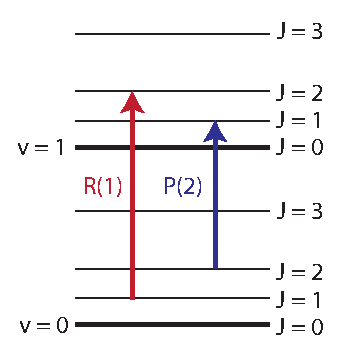
\includegraphics[width = 5 cm]{Transitions.eps}
\caption{Energy Transitions Diagram}
\label{fig:transitions}
\end{figure}

\section{Experimental Methods}

Data was recorded using a {SPECTROMETER NAME} FT IR spectrometer, using a high resolution and by averaging 64 scans to ensure usable, high-resolution data.

In order to correctly model the global precession of the data, both a cubic and a quadratic function were used and compared. These functions were defined as follows in \ref{eqn:fit}, with the quadratic version simply emitting the cubic term, i.e., $ D = 0$. Note that $D$ is just an arbitrary constant, whose physical meaning will be discussed later.

\begin{equation}
\label{eqn:fit}
\Delta S = \omega + \left( B_1 + B_0 \right) x + \left( B_1 - B_0 \right) x^2 + D x^4,
\end{equation}

\[ x = 
\begin{cases}
J + 1, \qquad J \in \textnormal{ R Branch }  \\
-J,    \qquad  \quad J \in \textnormal{ P Branch}
\end{cases}
\]

Data processing was done largely in \textsc{Python 3}, with \textsc{Mathematica} being used for some algebra and unit conversions. \textsc{SciPy}, several of its daughter packages, \textsc{NumPy} and \textsc{Matplotlib} were used extensively. Python code, raw data , {\LaTeX} files and illustrations can be found on \textsc{GitHub}\cite{GitHub}. Error handling was done natively within these packages.

\begin{figure*}[t]
\centering
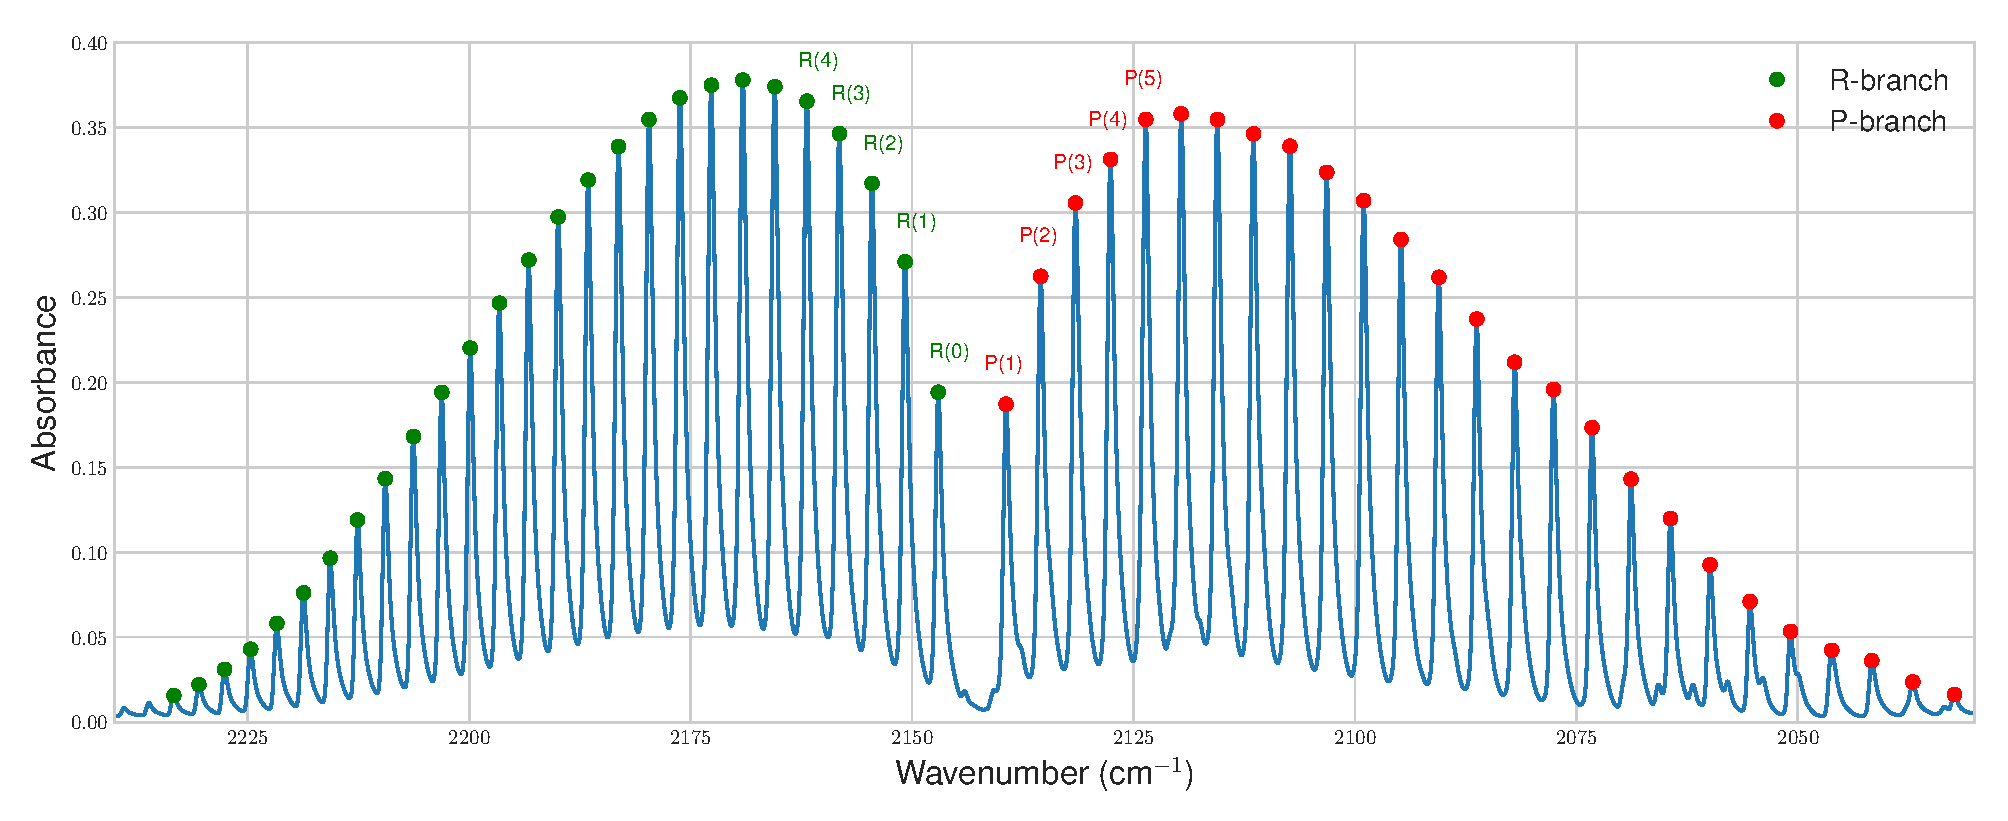
\includegraphics[width = 16 cm]{FormalExport.eps}
\caption{Fully assigned CO spectra, with some specific point labels omitted for clarity.}
\label{fig:spectra}
\end{figure*}

\section{Results}

Peaks were assigned as shown in figure \ref{fig:spectra}. The function in \ref{eqn:fit} was then fitted to extract $B_0$, $B_1$ and $\omega$ for both the quadratic and cubic case, with uncertainties from the fitting. These values were then used to calculate $B_e$ and $\alpha_e$ by solving $B_\nu = B_e - \alpha_e \left( \nu + 0.5 \right)$ for $\nu = 0$ and $1$ simultaneously, Then, equilibrium bond length was calculated using \ref{eqn:B}. More details can be found in the experimental notes\cite{notes}. The results are shown in table \ref{tab:results}, and the results of the cubic fit in figure \ref{fig:Cubic}.

\begin{figure}[H]
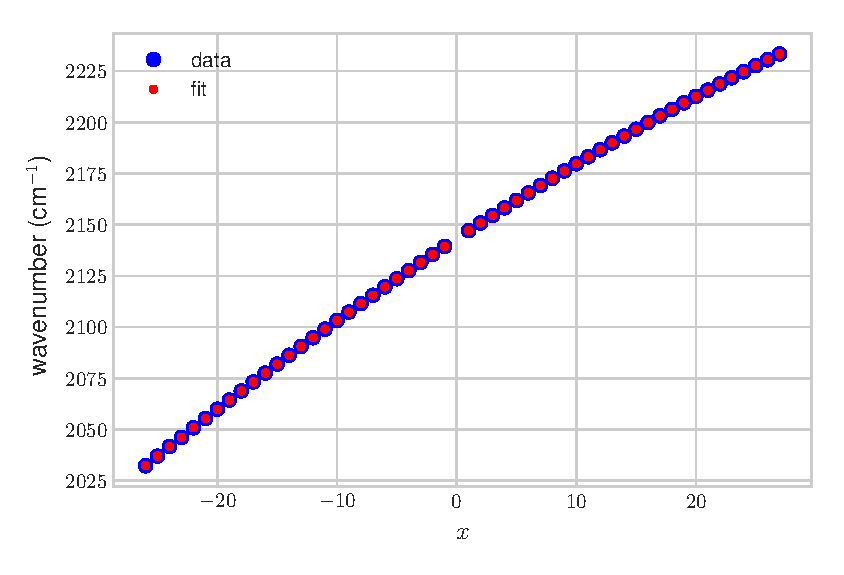
\includegraphics[width = 8 cm]{CubeFit.eps}
\caption{Cubic fit of Global Progression}
\label{fig:Cubic}
\end{figure}

\begin{table}[h]
\begin{tabular}{@{}lllllll@{}}
\toprule
                         & Cubic Fit    		& Quadratic Fit 		& Literature	&Units		& \\ \midrule
$B_0$          	& $1.9224(10)$       	& $1.8998(14)$         &$1.9225$ 	&cm$^{-1}$	& \\ 
$B_1$   		& $1.9054 (10)$      	& $1.9172(14)$         &$1.9051$	&cm$^{-1}$	& \\ 
$B_e$    		& $1.9312(10)$       	& $1.9260(14)$         &$1.9313$ 	&cm$^{-1}$	& \\
$\alpha_e$    	& $0.0174(15)$       	& $0.0175(19)$         &$0.0175$ 	&cm$^{-1}$	& \\ 
$\omega$ 	& $2143.190(13)$  	& $2143.192(32)$ 	&$2169.814$ 	&cm$^{-1}$	& \\ 
$r_e$   		& $1.1282(15)$       	& $1.1295(80)$         &$1.1283$	&\AA			& \\ \bottomrule
\end{tabular}
\caption{Experimental Constants Comparison \cite{NIST}\cite{MolSpectra}\cite{Education}}
\label{tab:results}
\end{table}

\pagebreak

To further investigate the two models, we should investigate their goodness of fit by calculating their respective sum of residuals. We find that the cubic and quadratic fits have a sum of $1234$ and $1234$ respectively, within the context of Absorbance values within about $0.05$ and $0.35$. This is pretty inconclusive by itself, so instead we can plot the residuals as in figure \ref{fig:Residuals}.

\begin{figure}[h]
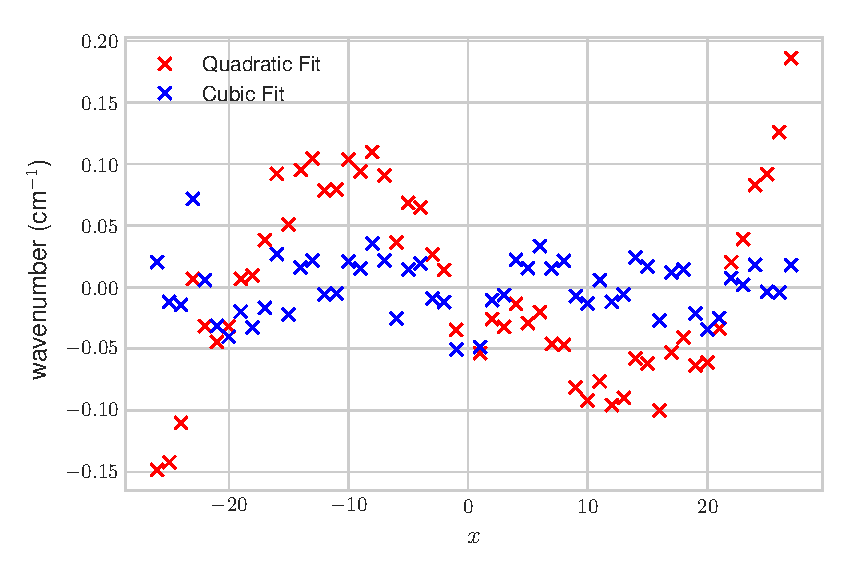
\includegraphics[width = 8 cm]{Residuals.eps}
\caption{Plot of Residuals}
\label{fig:Residuals}
\end{figure}

It should be clear that the residuals of the quadratic plot have a clear cubic pattern; they are far from random variations.This would appear to indicate that there is a systematic error in using the quadratic curve, and that therefore the cubic would be the most reflective of the physical system. This concurs with both the residuals and a comparison of experimental data with literature.

Finally, it is useful to attempt to fit a Boltzmann distribution to the intensity of the R branch to extract thermal data. Fitting equation \ref{eqn:Boltz} to the R branch data exclusively yields the following plot (figure \ref{fig:Thermals}) and a thermal value of $287$ K, or $12.8$ C.

\begin{equation}
I \left( J \right) = C \times \left( 2J + 1 \right) e^{ - B_0 J \left( J + 1 \right) /k_B T}
\label{eqn:Boltz}
\end{equation}

\begin{figure} [h]
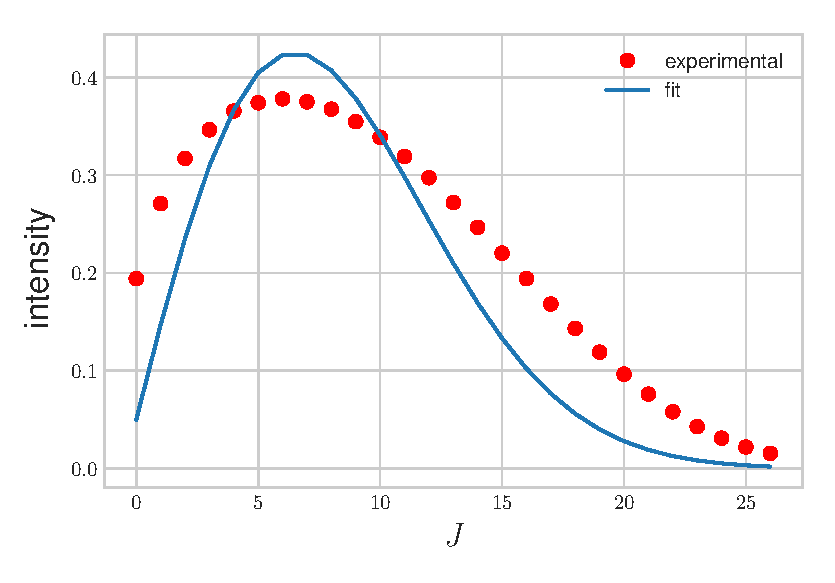
\includegraphics[width = 8 cm]{Thermal.eps}
\caption{Fitted Boltzmann Distribution to R Branch}
\label{fig:Thermals}
\end{figure}

\section{Discussion}

\lipsum[8]

\section{Conclusions}

You should finish with a succinct (1-2 sentence) statement of your key finding. It should be similar to (or even match) the conclusion you state in your abstract.

\begin{thebibliography}{99}

\bibitem[]{NIST} National Institute of Standards and Technology (NIST), U.S. Department of Commerce, 2021, {\it Carbon Monoxide}, NIST Chemistry WebBook, SRD 69, \href{https://webbook.nist.gov/cgi/cbook.cgi?ID=C630080}{accessed July 2022}. 

\bibitem[]{MolSpectra} Rank, D, St Pierre, A \& Wiggins, T 1965, ‘Rotational and Vibrational Constants of CO’, {\it Journal of Molecular Spectroscopy}, vol. 18, no. 4, \href{https://www.sciencedirect.com/science/article/abs/pii/0022285265900482}{pp. 418-427}.

\bibitem[]{Education} Mina-Camilde, N, Manzanares, C \& Caballero, J 1996, ‘Molecular Constants of Carbon Monoxide at v = 0, 1, 2, and 3: A Vibrational Spectroscopy Experiment in Physical Chemistry’, {\it Journal of Chemical Education}, vol. 73, no. 8, \href{https://doi.org/10.1021/ed073p804}{pp. 695-826}. 

\bibitem[]{textbook} T. Engel, 2019, {\it Quantum Chemistry and Spectroscopy}, 4th edn, Pearson Education, Inc, New York, USA.

\bibitem[]{GitHub} GitHub Repo go here

\bibitem[]{notes} Experimental Notes go here

\end{thebibliography}

\end{document}